\documentclass{article} % Define la clase del documento, en este caso, un artículo
\usepackage[letterpaper,margin=3cm]{geometry} % Configura el tamaño del papel y los márgenes del documento
\usepackage{graphicx} % Permite la inserción de imágenes
\usepackage[spanish]{babel}% Activar esta configuración para informes en español, ajusta el idioma del documento
\usepackage[usenames]{color} % Permite el uso de colores definidos por nombre en el documento
\usepackage{hyperref} % Habilita enlaces y referencias dentro del documento
\hypersetup{colorlinks=true, linkcolor = black, citecolor= black} % Configura el color de los enlaces y citas
\usepackage{booktabs} % Proporciona comandos para crear tablas de alta calidad
\usepackage{natbib} % Permite el uso de citas y referencias bibliográficas con diferentes estilos
\usepackage{tikz} % Permite la creación de gráficos y diagramas vectoriales directamente en LaTeX
\usepackage{float} % Para controlar la posición de los elementos flotantes, como imágenes, con la opción [H]
\usepackage{diagbox} % Permite crear celdas con líneas diagonales en tablas
\usepackage{listings} % Permite la inclusión y formateo de código fuente en el documento
\usepackage{xcolor} % Paquete para definir y usar colores en el documento
\usepackage{parskip} % Añade espacio entre párrafos en lugar de sangrías
\usepackage{fancyhdr} % Permite personalizar encabezados y pies de página
\usepackage{amsmath} % Proporciona una amplia variedad de entornos y comandos matemáticos

\pagestyle{fancy} % Usa el estilo fancyhdr
\fancyhf{} % Borra todos los encabezados y pies de página
\renewcommand{\headrulewidth}{0pt}
\renewcommand{\footrulewidth}{0pt} % Desactiva la línea horizontal predeterminada en el pie
\setlength{\headheight}{2cm} % Ajusta la altura del encabezado para hacer espacio para la línea
\fancyhead[L]{\raisebox{0.20cm}{\textbf{Hidrología}}} % Añade el texto en la parte izquierda del encabezado, subiéndolo ligeramente
\fancyhead[R]{\raisebox{0.1cm}{
\includegraphics[width=0.25\linewidth]{LOGO_UNIVERSIDAD.jpg}}} % Añade la imagen en la parte derecha del encabezado y súbela un poco
\fancyhead[C]{\rule{\textwidth}{0.6pt}} % Añade una línea horizontal superior centrada
\fancyfoot[C]{\rule{\textwidth}{0.6pt}} % Añade una línea horizontal en el pie de página centrada
\fancyfoot[R]{\raisebox{-1.5\baselineskip}{\thepage}} % Coloca el número de página a la derecha, con suficiente espacio debajo de la línea
\geometry{top=3cm, bottom=2.5cm} % Ajusta los márgenes superior e inferior

% Definición de colores al estilo Visual Studio Code
\definecolor{codegreen}{rgb}{0.25,0.49,0.48} % Comentarios
\definecolor{codegray}{rgb}{0.5,0.5,0.5} % Números y anotaciones
\definecolor{codepurple}{rgb}{0.58,0,0.82} % Palabras clave
\definecolor{backcolour}{rgb}{0.95,0.95,0.92} % Color de fondo

% Configuración del estilo de las celdas de código
\lstset{
    backgroundcolor=\color{backcolour},   % color de fondo; necesita que el paquete color o xcolor esté cargado
    commentstyle=\color{codegreen},       % estilo de comentarios
    keywordstyle=\color{codepurple},      % estilo de palabras clave
    numberstyle=\tiny\color{codegray},    % estilo de los números de línea
    stringstyle=\color{red},              % estilo de las cadenas de texto
    basicstyle=\ttfamily\small,           % estilo del texto básico
    breakatwhitespace=false,              % ajustes de líneas sólo en espacios en blanco
    breaklines=true,                      % ajustar las líneas si son muy largas
    captionpos=b,                         % posición de la leyenda (abajo)
    keepspaces=true,                      % preserva los espacios en el texto; útil si se usa monoespaciado
    numbers=left,                         % dónde poner los números de línea
    numbersep=5pt,                        % qué tan lejos están los números de línea del código
    showspaces=false,                     % mostrar espacios con subrayados particulares; reemplaza 'showstringspaces'
    showstringspaces=false,               % subrayar los espacios dentro de las cadenas solo
    showtabs=false,                       % mostrar tabulaciones en el código con subrayados particulares
    tabsize=2,                            % tamaños de tabulación a 2 espacios
    language=TeX,                         % lenguaje del código
    morecomment=[l]\#,                    % reconocer # como inicio de comentario en Python
    frame=single,                         % agregar un marco simple alrededor del código
    rulecolor=\color{black}               % color del marco
}

\begin{document}
%----------------------------------------------------------------------------------------
%   PORTADA
%Modificar desde aqui en adelante
%----------------------------------------------------------------------------------------
\begin{titlepage}%Inicio de la carátula, solo modificar los datos necesarios
\newcommand{\HRule}{\rule{\linewidth}{0.5mm}} 
\center 
%----------------------------------------------------------------------------------------
%	ENCABEZADO
%----------------------------------------------------------------------------------------

\includegraphics[width=10cm]{LOGO_UNIVERSIDAD.jpg}\\ % Si esta plantilla se copio correctamente, va a llevar la imagen del logo de la facultad.OBS: Es necesario incluir el paquete: graphicx
\vspace{3cm}
%----------------------------------------------------------------------------------------
%	SECCION DEL TITULO
%----------------------------------------------------------------------------------------
\HRule \\[0.4cm]
{ \huge \bfseries Tarea 1}\\[0.4cm] % Titulo del documento
{ \huge \bfseries Hidrología}\\[0.4cm] % Titulo del documento
\HRule \\[1.5cm]
 \vspace{5cm}
%----------------------------------------------------------------------------------------
%	SECCION DEL AUTOR
%----------------------------------------------------------------------------------------
\begin{flushright}
    { \textbf{Profesor:}\\
    Ricardo Gonzales\\
    \vspace{0.2cm}
    \textbf{Alumnos:}\\
    Bernardo Caprile Canala-Echevarría\\
    Pedro Tomás Valenzuela Bejares\\
    Felipe Alberto Vicencio Fossa \\
    Lukas Wolff Casanova\\
    \vspace{0.2cm}

}
\end{flushright}
\vspace{1cm}
%----------------------------------------------------------------------------------------
%	SECCION DE LA FECHA
%----------------------------------------------------------------------------------------
{\large \textbf{\today}}\\[2cm] % El comando \today coloca la fecha del dia, y esto se actualiza con cada compilacion, en caso de querer tener una fecha estatica, reemplazar el \today por la fecha deseada
\end{titlepage}
%----------------------------------------------------------------------------------------
%  INDICE
%----------------------------------------------------------------------------------------
\newpage
\tableofcontents
\thispagestyle{plain} % Deshabilita el encabezado en la página del índice
\thispagestyle{empty} % Deshabilita el número de página en la página del índice
\newpage

%Se puede agregar un indice de figuras si es nesesario
%\newpage
%\listoffigures 
%\thispagestyle{plain} % Deshabilita el encabezado en la página del índice %
%\thispagestyle{empty}
%\newpage
%----------------------------------------------------------------------------------------
%   ACÁ EMPIEZA EL INFORME
\setcounter{page}{1} % Reinicia el contador de páginas
%----------------------------------------------------------------------------------------
%Este es el formato a seguir para los titulos de las secciones

\section{Introducción}
En el presente informe se analizará la cuenca del Río Mapocho en Los Almendros (DGA 5722002), ubicada en la región central de Chile. El estudio tiene como objetivo evaluar las características hídricas de la cuenca, para poder entender el comportamiento y los recursos hídricos de esta.

Dentro de los objetivos específicos a lograr en este trabajo están determinar los parámetros físicos y climáticos representativos de la cuenca, analizar los caudales medios mensuales y anuales para identificar patrones y la variabilidad del flujo del agua, evaluar la evapotranspiración media anual y llevar a cabo un balance hidrológico para cuantificar la disponibilidad de agua.

Para esto, se procesarán datos de la Dirección General de Aguas (DGA) y el explorador de cuencas del CR2, de manera que se muestre un claro comportamiento hidrológico de la cuenca, facilitando así una futura gestión del agua.

\newpage
\section{Pregunta 1}

\subsection{Parámetros representativos de la cuenca}

\begin{table}[h!]
\centering
\begin{tabular}{>{\raggedright}p{6cm} p{8cm}}
\toprule
\textbf{Parámetro} & \textbf{Valor} \\
\midrule
Código DGA & 5722002 \\
Nombre de la estación & Río Mapocho en Los Almendros \\
Coordenadas geográficas del punto de salida & Latitud: -33.37, Longitud: -70.45 \\
Coordenadas UTM del punto de salida & Easting (X): 365109.50, Northing (Y): 6306754.64, Zona UTM: 19H \\ 
Elevación del punto de interés & 968 m s.n.m. \\
Área aportante & 638 km² \\
Elevación media de la cuenca & 2779 m s.n.m. \\
Elevación máxima de la cuenca & 5431 m s.n.m. \\
Trazado de la cuenca aportante & \textit{(Delimitación de la cuenca usando herramientas GIS)} \\
\bottomrule
\end{tabular}
\caption{Parámetros representativos de la cuenca del Río Mapocho en Los Almendros}
\label{table:parameters}
\end{table}

La cuenca 5722002 del Río Mapocho en Los Almendros, situada en la región central de Chile, tiene un área de 638 km². La precipitación anual media en esta cuenca es de 501 mm, según datos del CR2MET. La cuenca presenta un índice de aridez de 1.4 y varía en altitud desde los 968 m s.n.m. en el punto de salida hasta los 5431 m s.n.m. en su cota máxima, con una altitud media de 2779 m s.n.m.

\begin{itemize}
    \item \textbf{Zona 1:}
    \begin{itemize}
        \item \textbf{Código estación:} 5722002
        \item \textbf{Nombre estación:} Río Mapocho En Los Almendros
        \item \textbf{Ubicación:} Lat. -33.37, Lon. -70.45
        \item \textbf{Comienzo de observaciones:} 1999-08-01
        \item \textbf{Término de observaciones:} 2019-12-31
    \end{itemize}

    \item \textbf{Zona 2:}
    \begin{itemize}
        \item \textbf{Código estación:} 5720001
        \item \textbf{Nombre estación:} Río Molina Antes Junta San Francisco
        \item \textbf{Ubicación:} Lat. -33.37, Lon. -70.4
        \item \textbf{Comienzo de observaciones:} 2009-11-01
        \item \textbf{Término de observaciones:} 2019-12-31
    \end{itemize}

    \item \textbf{Zona 3:}
    \begin{itemize}
        \item \textbf{Código estación:} 5720003
        \item \textbf{Nombre estación:} La Ermita Central En Bocatoma
        \item \textbf{Ubicación:} Lat. -33.34, Lon. -70.36
        \item \textbf{Comienzo de observaciones:} 1987-05-01
        \item \textbf{Término de observaciones:} 2011-01-31
    \end{itemize}

    \newpage
    \item \textbf{Zona 4:}
    \begin{itemize}
        \item \textbf{Código estación:} 5721016
        \item \textbf{Nombre estación:} Río San Francisco Antes Junta Estero Yerba Loca
        \item \textbf{Ubicación:} Lat. -33.31, Lon. -70.36
        \item \textbf{Comienzo de observaciones:} 2013-04-01
        \item \textbf{Término de observaciones:} 2019-08-30
    \end{itemize}

    \item \textbf{Zona 5:}
    \begin{itemize}
        \item \textbf{Código estación:} 5721017
        \item \textbf{Nombre estación:} Estero Yerba Loca En Piedra Carvajal
        \item \textbf{Ubicación:} Lat. -33.22, Lon. -70.27
        \item \textbf{Comienzo de observaciones:} 2013-09-01
        \item \textbf{Término de observaciones:} 2019-12-31
    \end{itemize}
\end{itemize}

Estas estaciones han sido clave para obtener datos meteorológicos relevantes en distintas áreas de la cuenca, proporcionando información importante para la gestión del agua.

\newpage
\subsection{Información de Caudales Medios}

Se considerará un periodo de 30 años, comenzando el 1 de abril de 1993 y finalizando el 31 de marzo de 2023 el año hidrológico empieza en abril y termina en marzo. Los datos se obtuvieron \textbf{\citet{snia2024}}

\subsubsection{Caudales Medios Mensuales}

A continuación se presentan los caudales medios mensuales por estación a la salida de la cuenca (Zona 1):

\begin{table}[H]
    \centering
    \caption{Caudales Medios Mensuales}
    \vspace{0.2cm}
    \resizebox{\textwidth}{!}{%
    \begin{tabular}{|c|c|c|c|c|c|c|c|c|c|c|c|c|}
        \hline
        Año & Enero & Febrero & Marzo & Abril & Mayo & Junio & Julio & Agosto & Septiembre & Octubre & Noviembre & Diciembre \\
        \hline
        1993 & - & - & - & 3.46 & 18.46 & 6.87 & 4.93 & 5.10 & 5.44 & 6.45 & 6.72 & 7.20 \\
        1994 & 6.19 & 3.56 & 2.62 & 1.97 & 1.45 & 1.46 & 3.51 & 4.36 & 5.34 & 6.25 & 7.12 & 6.45 \\
        1995 & 5.26 & 3.11 & 2.14 & 1.84 & 1.58 & 2.30 & 2.20 & 2.72 & 4.76 & 4.77 & 5.73 & 4.47 \\
        1996 & 2.85 & 2.05 & 1.67 & 1.21 & 0.70 & 0.64 & 0.70 & 0.81 & 0.80 & 1.35 & 1.46 & 1.66 \\
        1997 & 2.32 & 1.71 & 1.44 & 0.96 & 1.36 & 12.47 & 6.21 & 10.41 & 16.96 & 17.75 & 22.07 & 19.74 \\
        1998 & 13.33 & 6.21 & 3.75 & 2.81 & 2.10 & 1.68 & 1.30 & 0.92 & 0.81 & 1.24 & 1.58 & 2.76 \\
        1999 & 2.60 & 2.58 & 1.54 & 1.07 & 0.77 & 0.70 & 1.04 & 1.65 & 8.57 & 6.94 & 7.48 & 5.69 \\
        2000 & 4.16 & 2.63 & 1.58 & 0.77 & 1.02 & 5.15 & 9.25 & 8.29 & 10.63 & 18.72 & 14.39 & 15.07 \\
        2001 & 7.18 & 3.75 & 1.20 & 1.07 & 2.33 & 2.07 & 8.85 & 15.05 & 10.04 & 13.33 & 11.16 & 11.71 \\
        2002 & 5.05 & 3.22 & 1.99 & 1.47 & 4.70 & 12.35 & 8.47 & 16.92 & 15.20 & 19.89 & 24.61 & 20.37 \\
        2003 & 14.94 & 9.28 & 5.74 & 3.93 & 3.08 & 3.52 & 3.64 & 3.41 & 3.87 & 5.78 & 5.78 & 4.65 \\
        2004 & 4.01 & 2.89 & 1.85 & 1.58 & 1.44 & 1.49 & 1.55 & 3.14 & 5.77 & 4.18 & 8.43 & 5.31 \\
        2005 & 3.64 & 2.95 & 2.42 & 1.63 & 2.08 & 10.79 & 5.58 & 14.06 & 12.29 & 16.35 & 22.97 & 18.37 \\
        2006 & 10.11 & 5.56 & 3.47 & 2.51 & 2.15 & 2.39 & 10.79 & 5.97 & 6.69 & 9.49 & 12.17 & 9.21 \\
        2007 & 5.33 & 3.07 & 2.54 & 2.13 & 1.93 & 2.31 & 2.90 & 2.52 & 4.61 & 6.55 & 5.38 & 3.97 \\
        2008 & 3.35 & 2.57 & 2.63 & 2.03 & 8.95 & 10.77 & 3.62 & 8.80 & 10.14 & 13.98 & 16.96 & 10.33 \\
        2009 & 5.94 & 2.98 & 2.27 & 1.86 & 1.95 & 1.97 & 2.38 & 4.28 & 14.20 & 11.77 & 10.56 & 9.12 \\
        2010 & 4.16 & 4.23 & 3.30 & 2.53 & 2.31 & 2.62 & 2.80 & 3.41 & 4.33 & 4.90 & 6.03 & 3.62 \\
        2011 & 2.74 & 2.15 & 1.44 & 1.45 & 1.12 & 1.20 & 1.37 & 1.77 & 4.24 & 4.41 & 3.66 & 3.87 \\
        2012 & 3.61 & 3.10 & 2.22 & 1.49 & 1.61 & 2.62 & 3.19 & 2.29 & 3.39 & 3.35 & 4.66 & 3.37 \\
        2013 & 3.59 & 2.98 & 1.83 & 1.41 & 1.43 & 1.82 & 1.82 & 2.69 & 3.53 & 4.56 & 4.32 & 3.43 \\
        2014 & 2.84 & 2.26 & 1.69 & 1.32 & 1.03 & 1.44 & 1.41 & 1.81 & 2.46 & 3.98 & 2.43 & 2.57 \\
        2015 & 2.40 & 2.20 & 2.20 & 1.45 & 1.26 & 1.11 & 1.21 & 4.03 & 4.82 & 7.44 & 8.63 & 7.99 \\
        2016 & 4.33 & 2.93 & 1.38 & 5.07 & 3.24 & - & 3.27 & 4.33 & 5.58 & 5.66 & 7.38 & 7.62 \\
        2017 & 5.56 & 2.84 & 2.00 & 2.32 & 2.34 & 3.05 & 2.65 & 2.70 & 4.75 & 6.00 & 5.39 & 4.57 \\
        2018 & 2.96 & 2.82 & 1.60 & 1.16 & 1.02 & 1.39 & 1.51 & 1.61 & 2.57 & 3.05 & 3.78 & 3.28 \\
        2019 & 3.06 & 2.04 & 1.63 & 1.12 & 0.86 & 1.14 & 1.16 & 1.10 & 1.37 & 1.17 & 1.41 & 1.77 \\
        2020 & 2.26 & 1.51 & 1.08 & 0.86 & 0.69 & 0.89 & 1.51 & 2.04 & 3.34 & 3.58 & 2.84 & 3.34 \\
        2021 & 3.01 & 3.21 & 1.99 & 1.04 & 0.96 & 0.89 & 0.84 & 1.35 & 2.40 & 2.19 & 1.67 & 1.84 \\
        2022 & 1.69 & 1.06 & 1.03 & 1.00 & 1.06 & 0.81 & 0.89 & 1.56 & 1.81 & 2.22 & - & - \\
        2023 & - & - & - & - & - & - & - & - & - & - & - & - \\
        \hline
    \end{tabular}%
    }
    \label{tab:caudales_mensuales}
    \vspace{0.2cm}
    \\Fuente: Estacion Rio Mapocho Los Almendros
\end{table}

\newpage
\subsubsection{Gráficos de Caudales Medios}
En la figura \ref{fig:caudales_mensual} se presentan los caudales medios mensuales de la cuenca del Río Mapocho.
\begin{figure}[h!]
    \centering
    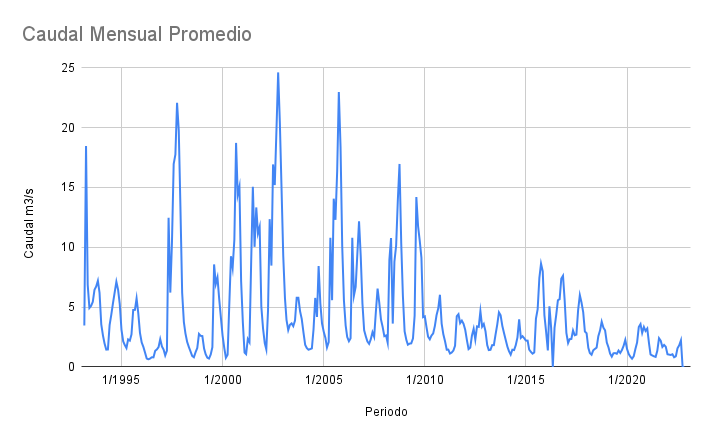
\includegraphics[width=0.8\textwidth]{GRAFICOS/Caudal Mensual Promedio.png}
    \caption{Caudales Medios Mensuales}
    \label{fig:caudales_mensual}
\end{figure}

\newpage
\subsubsection{Caudales Medios Temporada}

A continuación se presentan los caudales promedio por temporada, calculados a partir de los datos mensuales. La temporada se define como el período de un año hidrológico. Los valores reflejan el caudal medio durante cada temporada hidrológica desde 1993 hasta 2023.

\begin{table}[H]
    \centering
    \small % Reduce el tamaño de la fuente de la tabla
    \caption{Caudales Medios por Temporada}
    \vspace{0.2cm}
    \begin{tabular}{|c|c|}
        \hline
        \textbf{Temporada} & \textbf{Caudal Promedio (m³/s)} \\
        \hline
        1993-1994 & 6.41666667 \\
        1994-1995 & 4.035 \\
        1995-1996 & 3.07833333 \\
        1996-1997 & 1.23333333 \\
        1997-1998 & 10.935 \\
        1998-1999 & 1.82666667 \\
        1999-2000 & 3.52333333 \\
        2000-2001 & 7.95166667 \\
        2001-2002 & 7.15583333 \\
        2002-2003 & 12.8283333 \\
        2003-2004 & 3.8675 \\
        2004-2005 & 3.49166667 \\
        2005-2006 & 10.2716667 \\
        2006-2007 & 6.02583333 \\
        2007-2008 & 3.40416667 \\
        2008-2009 & 8.06416667 \\
        2009-2010 & 5.815 \\
        2010-2011 & 3.24 \\
        2011-2012 & 2.66833333 \\
        2012-2013 & 2.86416667 \\
        2013-2014 & 2.65 \\
        2014-2015 & 2.10416667 \\
        2015-2016 & 3.88166667 \\
        2016-2017 & 4.77727273 \\
        2017-2018 & 3.42916667 \\
        2018-2019 & 2.175 \\
        2019-2020 & 1.32916667 \\
        2020-2021 & 2.275 \\
        2021-2022 & 1.41333333 \\
        2022-2023 & 1.33571429 \\
        \hline
    \end{tabular}
    \label{tab:caudales_temporada}
    \vspace{0.2cm}
    \\Fuente: Estacion Rio Mapocho Los Almendros
\end{table}

\newpage
\subsubsection{Gráfico de Caudales Anuales}

En la figura \ref{fig:caudales_anual} se presentan los caudales medios anuales de la cuenca del Río Mapocho.
\begin{figure}[h!]
    \centering
    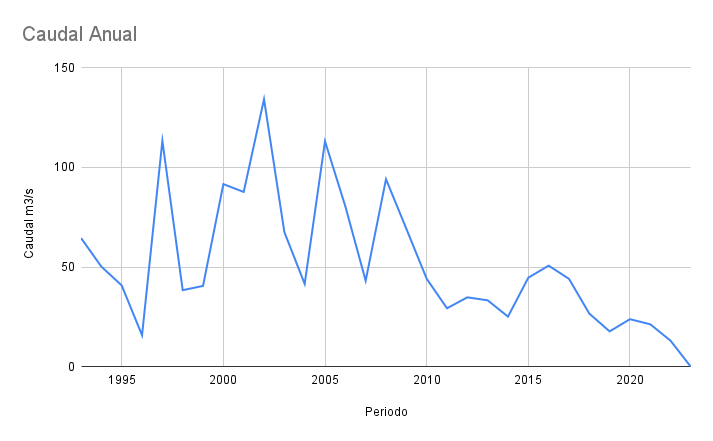
\includegraphics[width=0.8\textwidth]{GRAFICOS/Caudal Anual.png}
    \caption{Caudales Medios Anuales}
    \label{fig:caudales_anual}
\end{figure}

\newpage
\subsubsection{Promedio y desviación estandar de caudales máximos  diarios}

\begin{table}[h]
    \centering
    \caption{Máximos anuales, promedios y desviaciones estándar (1993-2022)}
    \begin{tabular}{|c|c|c|c|}
    \hline
    \textbf{Año} & \textbf{Máximo anual} & \textbf{Promedio} & \textbf{Desviación estándar} \\ \hline
    1993 & 18.46 & 7.18 & 4.39 \\ \hline
    1994 & 7.12 & 4.19 & 2.06 \\ \hline
    1995 & 5.73 & 3.41 & 1.49 \\ \hline
    1996 & 2.85 & 1.33 & 0.67 \\ \hline
    1997 & 22.07 & 9.45 & 8.11 \\ \hline
    1998 & 13.33 & 3.21 & 3.53 \\ \hline
    1999 & 8.57 & 3.39 & 2.93 \\ \hline
    2000 & 18.72 & 7.64 & 6.08 \\ \hline
    2001 & 15.05 & 7.31 & 5.06 \\ \hline
    2002 & 24.61 & 11.19 & 8.09 \\ \hline
    2003 & 14.94 & 5.64 & 3.40 \\ \hline
    2004 & 8.43 & 3.47 & 2.18 \\ \hline
    2005 & 22.97 & 9.43 & 7.37 \\ \hline
    2006 & 12.17 & 6.71 & 3.59 \\ \hline
    2007 & 6.55 & 3.60 & 1.53 \\ \hline
    2008 & 16.96 & 7.84 & 4.95 \\ \hline
    2009 & 14.20 & 5.77 & 4.47 \\ \hline
    2010 & 6.03 & 3.69 & 1.10 \\ \hline
    2011 & 4.41 & 2.45 & 1.27 \\ \hline
    2012 & 4.66 & 2.91 & 0.90 \\ \hline
    2013 & 4.56 & 2.78 & 1.11 \\ \hline
    2014 & 3.98 & 2.10 & 0.82 \\ \hline
    2015 & 8.63 & 3.73 & 2.83 \\ \hline
    2016 & 7.62 & 4.23 & 2.25 \\ \hline
    2017 & 6.00 & 3.68 & 1.46 \\ \hline
    2018 & 3.78 & 2.23 & 0.94 \\ \hline
    2019 & 3.06 & 1.49 & 0.60 \\ \hline
    2020 & 3.58 & 2.00 & 1.06 \\ \hline
    2021 & 3.21 & 1.78 & 0.81 \\ \hline
    2022 & 2.22 & 1.09 & 0.67 \\ \hline
    \end{tabular}\\
    Fuente: Estacion Rio Mapocho Los Almendros
\end{table}
    


\newpage
\subsection{Información de Precipitaciones Medias}
A continuación se presentan las precipitaciones totales por cada estación mensualmente, de esta forma, es posible obtener la precipitación media mensual. 

Para obtener las precipitaciones, se utilizó la base de datos \textbf{\citet{reportesSNIA}}

\subsubsection{Estación Río Mapocho En Los Almendros}

\begin{table}[H]
    \centering
    \caption{Precipitaciones Estación Río Mapocho En Los Almendros}
    \vspace{0.2cm}
    \resizebox{\textwidth}{!}{%
    \begin{tabular}{|c|c|c|c|c|c|c|c|c|c|c|c|c|}
        \hline
        Año & Enero & Febrero & Marzo & Abril & Mayo & Junio & Julio & Agosto & Septiembre & Octubre & Noviembre & Diciembre \\
        \hline
        1999 & - & - & - & 0.00 & 0.00 & 0.00 & 122.10 & 84.70 & 24.40 & 0.00 & 0.00 & 0.00 \\
        2000 & 9.80 & 0.00 & 37.60 & 30.40 & 308.50 & 76.90 & 14.60 & 123.50 & 10.60 & 15.30 & 0.00 & 0.00 \\
        2001 & 0.00 & 0.00 & 15.70 & 27.10 & 68.40 & 10.50 & 186.20 & 78.80 & 48.90 & 21.10 & 0.70 & 0.00 \\
        2002 & 1.30 & 0.00 & 32.20 & 38.30 & 158.70 & 193.10 & 96.20 & 114.80 & 45.00 & 16.40 & 3.80 & 1.70 \\
        2003 & 11.30 & 0.00 & 0.30 & 30.80 & 23.20 & 76.70 & 7.50 & 18.20 & 0.00 & 12.10 & 0.00 & 0.00 \\
        2004 & 1.50 & 20.10 & 40.90 & 20.50 & 55.70 & 88.60 & 73.10 & 68.20 & 20.50 & 98.90 & 0.00 & 0.00 \\
        2005 & 8.50 & 0.00 & 16.60 & 7.30 & 76.60 & 148.70 & 41.00 & 227.70 & 53.10 & 64.00 & 11.90 & 0.00 \\
        2006 & 0.00 & 0.00 & 0.00 & 0.80 & 5.00 & 74.10 & 219.90 & 46.90 & 10.00 & 58.90 & 2.20 & 0.00 \\
        2007 & 0.00 & 41.70 & 9.10 & 6.40 & 89.00 & 60.00 & 53.00 & 0.50 & 0.00 & 0.00 & 0.00 & 0.00 \\
        2008 & 0.00 & 16.00 & 5.80 & 163.80 & 62.40 & 31.90 & 164.50 & 9.50 & 0.30 & 0.00 & 0.00 & 0.00 \\
        2009 & 0.00 & 3.00 & 0.50 & 0.00 & 10.80 & 106.40 & 41.60 & 115.40 & 101.50 & 20.60 & 0.00 & 0.00 \\
        2010 & 0.00 & 0.00 & 0.00 & 0.80 & 59.30 & 90.80 & 44.80 & 3.40 & 39.30 & 20.50 & 69.80 & 0.80 \\
        2011 & 0.00 & 3.70 & 0.00 & 0.00 & 49.10 & 56.70 & 37.20 & 13.30 & 17.20 & 2.40 & 0.00 & 0.00 \\
        2012 & 0.00 & 0.00 & 38.30 & 39.80 & 73.80 & 8.40 & 61.40 & 5.00 & 54.00 & 5.80 & 38.00 & 0.00 \\
        2013 & 1.10 & 1.60 & 0.00 & 0.00 & 73.80 & 24.60 & 9.00 & 34.40 & 17.20 & 0.20 & 0.00 & 0.00 \\
        2014 & 0.40 & 0.10 & 0.00 & 0.40 & 15.00 & 73.60 & 25.20 & 50.80 & 33.40 & 0.40 & 8.40 & 0.00 \\
        2015 & 0.00 & 3.20 & 22.20 & 0.20 & 0.00 & 31.60 & 84.00 & 43.80 & 57.40 & 9.00 & 0.00 & 0.00 \\
        2016 & 0.00 & 0.00 & 107.60 & 31.00 & 48.00 & 0.00 & 0.40 & 0.00 & 0.00 & 0.00 & 0.00 & 0.00 \\
        2017 & 0.00 & 0.00 & 0.00 & 7.20 & 56.60 & 1.80 & 0.00 & 0.00 & 0.00 & 0.00 & 0.00 & 0.00 \\
        2018 & 0.00 & 0.00 & 1.40 & 0.00 & 1.00 & 29.40 & 21.60 & 30.40 & 0.00 & 0.00 & 0.00 & 0.00 \\
        2019 & 0.00 & 0.00 & 0.00 & 0.00 & 6.80 & 20.00 & 22.00 & 9.00 & 0.20 & 0.00 & 0.00 & 0.00 \\
        2020 & 0.00 & 0.00 & 0.00 & 1.80 & 5.80 & 58.60 & 70.00 & 15.80 & 0.40 & 0.00 & 0.00 & 0.00 \\
        2021 & - & - & - & - & - & - & - & - & - & - & - & - \\
        2022 & - & - & - & - & - & - & - & - & - & - & - & - \\
        2023 & - & - & - & - & - & - & - & - & - & - & - & - \\
        \hline
    \end{tabular}%
    }
    \label{tab:precipitaciones_rio_mapocho}
    \vspace{0.2cm}
    \\Fuente: Estacion Rio Mapocho Los Almendros
\end{table}


\subsubsection{Estación Río Molina Antes de junta con San Francisco}

\begin{table}[H]
    \centering
    \caption{Precipitaciones Estación Río Molina Antes Junta San Francisco}
    \vspace{0.2cm}
    \resizebox{\textwidth}{!}{%
    \begin{tabular}{|c|c|c|c|c|c|c|c|c|c|c|c|c|}
        \hline
        Año & Enero & Febrero & Marzo & Abril & Mayo & Junio & Julio & Agosto & Septiembre & Octubre & Noviembre & Diciembre \\
        \hline
        2009 & - & - & - & - & - & - & - & - & - & - & 0.9 & 0.0 \\
        2010 & 0.0 & 0.0 & 0.0 & 1.7 & 68.5 & 109.3 & 26.1 & 1.5 & 36.2 & 20.4 & 60.7 & 2.9 \\
        2011 & 0.1 & 12.5 & - & 2.4 & 0.0 & 29.4 & 59.0 & 37.8 & 13.9 & 17.1 & 2.5 & 0.0 \\
        2012 & 5.4 & 0.0 & 0.0 & 42.7 & 50.2 & 91.3 & 7.5 & 65.6 & 4.9 & 52.6 & 5.5 & 34.7 \\
        2013 & 2.8 & 8.4 & 0.0 & 1.0 & 119.4 & 47.6 & 16.7 & 56.7 & 24.9 & 3.2 & 0.0 & 0.2 \\
        2014 & 0.4 & 1.9 & 2.6 & 1.0 & 19.3 & 97.5 & 26.9 & 72.9 & 37.1 & 0.3 & 10.0 & 0.5 \\
        2015 & 0.0 & 12.8 & 44.0 & 0.0 & 0.8 & 0.0 & 55.9 & 132.5 & 64.8 & 63.4 & 9.4 & 0.0 \\
        2016 & 6.9 & 0.0 & 0.0 & 132.0 & 62.8 & 64.8 & 38.7 & 0.8 & 7.5 & 47.5 & 6.3 & 56.5 \\
        2017 & 0.0 & 0.2 & 0.5 & 13.8 & 109.4 & 88.7 & 5.2 & 0.0 & 0.0 & 0.0 & 0.0 & 0.0 \\
        2018 & 0.1 & 0.0 & 1.8 & 0.0 & 13.1 & 0.1 & 0.0 & 20.2 & 0.0 & 0.0 & 0.0 & 0.0 \\
        2019 & 0.0 & 0.0 & 0.3 & 0.0 & 18.6 & 27.0 & 0.4 & 0.0 & 0.0 & 20.6 & 0.0 & 0.0 \\
        2020 & 0.0 & 0.0 & 0.0 & 3.2 & 6.0 & 97.4 & 55.3 & 13.9 & 0.0 & 0.0 & 0.0 & 0.0 \\
        2021 & 0.0 & 0.0 & 0.0 & 0.0 & 0.0 & 0.0 & 0.0 & 0.0 & 0.0 & 0.0 & 0.0 & 0.0 \\
        2022 & 0.0 & 0.0 & 0.0 & 0.0 & 0.0 & 0.0 & 0.0 & 0.0 & 0.0 & 0.0 & 0.0 & 0.0 \\
        2023 & 0.0 & 0.0 & 0.0 & 0.0 & - & - & - & - & - & - & - & - \\
        \hline
    \end{tabular}%
    }
    \label{tab:precipitaciones_rio_molina}
    \vspace{0.2cm}
    \\Funete: Estacion Rio Molina Antes Junta San Francisco
\end{table}

\subsubsection{Estación La Ermita Central En Bocatoma}

La estación no presenta registros de precipitaciones

\subsubsection{Estación Río San Francisco Antes de junta con Estero Yerba Loca}

\begin{table}[H]
    \centering
    \caption{Precipitaciones Estación Río San Francisco Antes Junta Estero Yerba Loca}
    \vspace{0.2cm}
    \resizebox{\textwidth}{!}{%
    \begin{tabular}{|c|c|c|c|c|c|c|c|c|c|c|c|c|}
        \hline
        Año & Enero & Febrero & Marzo & Abril & Mayo & Junio & Julio & Agosto & Septiembre & Octubre & Noviembre & Diciembre \\
        \hline
        2013 & - & - & - & 4.8 & 154.4 & 66.0 & 39.0 & 75.0 & 36.4 & 3.4 & 1.6 & 0.8 \\
        2014 & 3.0 & 12.2 & 2.2 & 1.6 & 29.8 & 118.0 & 14.4 & 64.4 & 28.8 & 4.4 & 24.6 & 0.4 \\
        2015 & 0.0 & 21.2 & 0.0 & 0.0 & 4.0 & 4.0 & 0.0 & 94.0 & 354.6 & 315.0 & 138.6 & 107.6 \\
        2016 & 10.9 & 0.0 & 0.0 & 119.9 & 167.4 & 104.0 & 56.5 & 52.2 & 52.2 & 0.0 & 56.7 & 64.0 \\
        2017 & 0.0 & 0.1 & 1.3 & 17.4 & 108.4 & 142.2 & 50.0 & 15.5 & 15.5 & 0.0 & 0.0 & 0.0 \\
        2018 & 0.0 & 0.0 & 0.0 & 0.0 & 0.0 & 20.3 & 20.3 & 1.3 & 11.0 & 9.7 & 0.0 & 0.0 \\
        2019 & 0.0 & 0.0 & 0.0 & 0.0 & 7.2 & 26.7 & 10.3 & 0.5 & 0.0 & 11.6 & 0.1 & 0.0 \\
        2020 & 0.0 & 0.0 & 0.0 & 5.4 & 8.8 & 109.2 & 44.4 & 13.6 & 0.0 & 0.0 & 0.0 & 0.0 \\
        \hline
    \end{tabular}%
    }
    \label{tab:precipitaciones_rio_san_francisco}
    \vspace{0.2cm}
    \\Fuente: Estacion Rio San Francisco Antes Junta Estero Yerba Loca
\end{table}

\subsubsection{Estacion Estero Yerba Loca En Piedra Carvajal}

La toma de datos de esta estación no fue regular, por lo tanto, no se considerará para efectos de cálculo.

\begin{table}[H]
    \centering
    \caption{Precipitaciones Estación Estero Yerba Loca en Piedra Carvajal}
    \vspace{0.2cm}
    \resizebox{\textwidth}{!}{%
    \begin{tabular}{|c|c|c|c|c|c|c|c|c|c|c|c|c|}
        \hline
        Año & Enero & Febrero & Marzo & Abril & Mayo & Junio & Julio & Agosto & Septiembre & Octubre & Noviembre & Diciembre \\
        \hline
        2011 & - & - & - & 0.0 & 0.0 & 0.0 & 0.0 & 0.0 & 0.0 & 0.0 & 0.0 & 0.0 \\
        2012 & 0.00 & 0.00 & 0.00 & 0.00 & 0.00 & 0.00 & 0.00 & 0.00 & 0.00 & 0.00 & 0.00 & 0.00 \\
        2013 & 0.00 & 0.00 & 0.00 & 0.00 & 0.00 & 0.00 & 0.00 & 0.00 & 9.30 & 6.00 & 6.10 & 0.00 \\
        2014 & 0.00 & 0.00 & 0.00 & 0.00 & 0.00 & 0.00 & 0.00 & 0.00 & 0.00 & 6.00 & 1.90 & 0.00 \\
        2015 & 0.00 & 11.00 & 32.90 & 0.0 & 0.0 & 0.0 & 0.0 & 11.90 & 0.0 & 0.0 & 2.80 & 0.0 \\
        2016 & 0.00 & 0.00 & 0.00 & 0.00 & 0.00 & 0.00 & 0.90 & 0.00 & 0.00 & 0.00 & 0.00 & 0.00 \\
        2017 & 0.00 & 0.00 & 11.80 & 17.90 & 25.10 & 1.40 & 2.10 & 0.00 & 0.00 & 0.00 & 0.00 & 0.00 \\
        2018 & 18.50 & 1.40 & 8.60 & 0.40 & 9.90 & 4.40 & 76.60 & 2.50 & 0.00 & 0.00 & 0.00 & 0.00 \\
        2019 & 1.70 & 2.10 & 0.80 & 2.70 & 2.30 & 3.50 & 2.40 & 0.00 & 1.80 & 0.00 & 7.00 & 0.00 \\
        2020 & 0.30 & 0.00 & 3.40 & 1.50 & 8.10 & 2.70 & 0.20 & 0.00 & 0.00 & 0.00 & 0.00 & 0.00 \\
        2021 & 0.00 & 0.00 & 0.00 & 0.00 & 0.00 & 0.00 & 0.00 & 0.00 & 0.00 & 0.00 & 0.00 & 0.00 \\
        2022 & 0.00 & 0.00 & 0.00 & 0.00 & 0.00 & 0.00 & 0.00 & 0.00 & 0.00 & 0.00 & 0.00 & 0.00 \\
        2023 & 0.00 & 0.00 & 0.00 & - & - & - & - & - & - & - & - & - \\
        \hline
    \end{tabular}%
    }
    \label{tab:precipitaciones_estero_yerba_loca}
    \vspace{0.2cm}
    \\Fuente: Estacion Estero Yerba Loca en Piedra Carvajal
\end{table}

\newpage
\subsubsection{Precipitaciones promedio mensuales según las 5 zonas}

\begin{table}[H]
    \centering
    \caption{Precipitaciones Promedio Mensuales según las 5 zonas}
    \vspace{0.2cm}
    \resizebox{\textwidth}{!}{%
    \begin{tabular}{|c|c|c|c|c|c|c|c|c|c|c|c|c|}
    \hline
    Año & Enero & Febrero & Marzo & Abril & Mayo & Junio & Julio & Agosto & Septiembre & Octubre & Noviembre & Diciembre \\
    \hline
    1993 & - & - & - & - & - & - & - & - & - & - & - & - \\
    1994 & - & - & - & - & - & - & - & - & - & - & - & - \\
    1995 & - & - & - & - & - & - & - & - & - & - & - & - \\
    1996 & - & - & - & - & - & - & - & - & - & - & - & - \\
    1997 & - & - & - & - & - & - & - & - & - & - & - & - \\
    1998 & - & - & - & - & - & - & - & - & - & - & - & - \\
    1999 & 0.00 & 0.00 & 0.00 & 122.10 & 84.70 & 24.40 & 0.00 & 0.00 & 0.00 & - & - & - \\
    2000 & 9.80 & 0.00 & 37.60 & 30.40 & 308.50 & 76.90 & 14.60 & 123.50 & 10.60 & 15.30 & 0.00 & 0.00 \\
    2001 & 0.00 & 0.00 & 15.70 & 27.10 & 68.40 & 10.50 & 186.20 & 78.80 & 48.90 & 21.10 & 0.70 & 0.00 \\
    2002 & 1.30 & 0.00 & 32.20 & 38.30 & 158.70 & 193.10 & 96.20 & 114.80 & 45.00 & 16.40 & 3.80 & 1.70 \\
    2003 & 11.30 & 0.00 & 0.30 & 30.80 & 23.20 & 76.70 & 7.50 & 18.20 & 0.00 & 12.10 & 0.00 & 0.00 \\
    2004 & 1.50 & 20.10 & 40.90 & 20.50 & 55.70 & 88.60 & 73.10 & 68.20 & 20.50 & 98.90 & 0.00 & 0.00 \\
    2005 & 8.50 & 0.00 & 16.60 & 7.30 & 76.60 & 148.70 & 41.00 & 227.70 & 53.10 & 64.00 & 11.90 & 0.00 \\
    2006 & 0.00 & 0.00 & 0.00 & 0.80 & 5.00 & 74.10 & 219.90 & 46.90 & 10.00 & 58.90 & 2.20 & 0.00 \\
    2007 & 0.00 & 41.70 & 9.10 & 6.40 & 89.00 & 60.00 & 53.00 & 0.50 & 0.00 & 0.00 & 0.00 & 0.00 \\
    2008 & 0.00 & 16.00 & 5.80 & 163.80 & 62.40 & 31.90 & 164.50 & 9.50 & 0.30 & 0.00 & 0.00 & 0.00 \\
    2009 & 0.00 & 3.00 & 0.50 & 0.00 & 10.80 & 106.40 & 41.60 & 115.40 & 101.50 & 20.60 & 0.00 & 0.00 \\
    2010 & 0.00 & 0.00 & 0.00 & 0.80 & 59.30 & 90.80 & 44.80 & 3.40 & 39.30 & 20.50 & 69.80 & 0.80 \\
    2011 & 0.00 & 3.70 & 0.00 & 0.00 & 24.55 & 56.70 & 48.10 & 13.30 & 17.20 & 2.40 & 0.00 & 0.00 \\
    2012 & 0.00 & 0.00 & 19.15 & 39.80 & 73.80 & 8.40 & 61.40 & 5.00 & 54.00 & 5.80 & 38.00 & 0.00 \\
    2013 & 1.10 & 1.60 & 0.00 & 0.50 & 73.80 & 45.30 & 24.00 & 54.70 & 17.20 & 0.20 & 0.00 & 0.00 \\
    2014 & 1.70 & 0.10 & 0.00 & 0.70 & 15.00 & 95.80 & 25.20 & 50.80 & 33.40 & 0.40 & 9.20 & 0.00 \\
    2015 & 0.00 & 3.20 & 22.07 & 0.07 & 2.00 & 11.87 & 42.00 & 68.90 & 57.40 & 162.00 & 0.00 & 0.00 \\
    2016 & 0.00 & 0.00 & 35.87 & 81.50 & 48.00 & 52.00 & 0.40 & 0.00 & 0.00 & 0.00 & 0.00 & 32.00 \\
    2017 & 0.00 & 0.00 & 0.00 & 7.20 & 56.60 & 1.80 & 25.00 & 0.00 & 0.00 & 0.00 & 0.00 & 0.00 \\
    2018 & 0.00 & 0.00 & 0.70 & 0.00 & 0.50 & 29.40 & 10.80 & 30.40 & 3.67 & 0.00 & 0.00 & 0.00 \\
    2019 & 0.00 & 0.00 & 0.00 & 0.00 & 6.80 & 23.50 & 22.00 & 4.50 & 0.07 & 0.00 & 0.00 & 0.00 \\
    2020 & 0.00 & 0.00 & 0.00 & 1.80 & 5.90 & 58.60 & 70.00 & 15.80 & 0.20 & 0.00 & 0.00 & 0.00 \\
    2021 & - & - & - & - & - & - & - & - & - & - & - & - \\
    2022 & - & - & - & - & - & - & - & - & - & - & - & - \\
    2023 & - & - & - & - & - & - & - & - & - & - & - & - \\
    \hline
    \end{tabular}%
    }
    \label{tab:precipitaciones_promedio}
    \vspace{0.2cm}
    \\Fuente: Datos de precipitaciones de las estaciones mencionadas
\end{table}

Los datos de precipitaciones promedio mensuales son aplicables en diferentes zonas según los períodos especificados: Zona 1 cubre desde abril de 1993 hasta septiembre de 2022; Zona 2, desde enero de 2010 hasta agosto de 2020; y Zona 4, desde abril de 2013 hasta agosto de 2019. No hay datos aplicables para las zonas 3 y 5 en los períodos considerados. Estos datos permiten analizar las variaciones y patrones de precipitación en las áreas y tiempos indicados.

\newpage
\subsubsection{Gráfico de precipitaciones mensuales promedio}
En la figura \ref{fig:presipitaciones_mensuales} se muestra el gráfico de precipitaciones mensuales promedio en las zonas mencionadas.
\begin{figure}[h!]
    \centering
    \includegraphics[width=0.8\textwidth]{GRAFICOS/Precipitación Mensual promedio.png}
    \caption{Precipitaciones Medias Mensuales}
    \label{fig:presipitaciones_mensuales}
\end{figure}

\newpage

\subsubsection{Precipitaciones promedio anuales según las 5 zonas}

\begin{table}[ht]
    \centering
    \caption{Precipitaciones Promedio Anuales (Según Zonas)}
    \vspace{0.2cm}
    \begin{tabular}{|c|c|}
        \hline
        \textbf{Periodo} & \textbf{Precipitaciones (mm)} \\
        \hline
        1993-1994 & 0.00 \\
        1994-1995 & 0.00 \\
        1995-1996 & 0.00 \\
        1996-1997 & 0.00 \\
        1997-1998 & 0.00 \\
        1998-1999 & 0.00 \\
        1999-2000 & 278.60 \\
        2000-2001 & 595.50 \\
        2001-2002 & 475.20 \\
        2002-2003 & 679.60 \\
        2003-2004 & 231.00 \\
        2004-2005 & 450.60 \\
        2005-2006 & 630.30 \\
        2006-2007 & 468.60 \\
        2007-2008 & 230.70 \\
        2008-2009 & 435.90 \\
        2009-2010 & 396.30 \\
        2010-2011 & 333.20 \\
        2011-2012 & 181.40 \\
        2012-2013 & 288.90 \\
        2013-2014 & 217.50 \\
        2014-2015 & 255.77 \\
        2015-2016 & 380.10 \\
        2016-2017 & 213.90 \\
        2017-2018 & 91.30 \\
        2018-2019 & 74.77 \\
        2019-2020 & 56.87 \\
        2020-2021 & 152.30 \\
        2021-2022 & 0.00 \\
        2022-2023 & 0.00 \\
        \hline
    \end{tabular}
    \label{tab:precipitaciones_anuals}
    \vspace{0.2cm}
    \\Fuente: Datos de precipitaciones de las estaciones mencionadas
\end{table}

\newpage
\subsubsection{Gráfico de precipitaciones anuales promedio}

En la figura \ref{fig:precipitaciones_anuales} se muestra el gráfico de precipitaciones anuales promedio en las zonas mencionadas.
\begin{figure}[h!]
    \centering
    \includegraphics[width=0.8\textwidth]{GRAFICOS/Precipitación Anual.png}
    \caption{Precipitaciones Anuales Promedio}
    \label{fig:precipitaciones_anuales}
\end{figure}


\newpage
\subsection{Balance Hidrológico}

El balance hidrológico se describe matemáticamente con la siguiente ecuación:

\begin{equation}
    \frac{dS}{dt} = X - Y
\end{equation}

donde:

\begin{itemize}
    \item $X$ representa las entradas de agua al sistema (como la precipitación, P).
    \item $Y$ representa las salidas de agua del sistema (como la evaporación, E, y el caudal, Q).
    \item $\frac{dS}{dt}$ es la tasa de variación del almacenamiento de agua en el sistema con respecto al tiempo.
\end{itemize}

\subsubsection{Simplificación de la Ecuación}

La ecuación del balance hidrológico puede simplificarse en un contexto de largo plazo o cuando se consideran promedios anuales, donde el cambio en el almacenamiento ($\frac{dS}{dt}$) tiende a cero, resultando en:

\begin{equation}
    P = Q + ET
    \label{eq:evaporacion}
\end{equation}

donde:
\begin{itemize}
    \item $P$ es la precipitación anual media (501 mm en este estudio).
    \item $Q$ es el caudal medio que puede ser calculado en términos mensuales, anuales o diarios.
    \item $ET$ es la evapotranspiración, que incluye tanto la evaporación del suelo y cuerpos de agua como la transpiración de las plantas.
\end{itemize}

\subsubsection{Cálculo de la Evapotranspiración}

La evapotranspiración (ET) teórica se puede calcular utilizando la fórmula de Penman-Monteith o métodos simplificados dependiendo de la disponibilidad de datos. En este estudio, se ha considerado:

\begin{equation}
    ET = f(P, T, Q)
\end{equation}

donde $T$ es la temperatura media, que se puede obtener mediante el análisis de isolíneas y otros datos meteorológicos.

\subsection{Cálculo de la Evaporación Media Anual y Mensual}

Para el analisis de evaporacion, se analizaran los datos anuales y mensuales.

\subsubsection{Evaporación Media Anual}

A continuación se muestra la evaporación media mensual, para la que se consideraron solo los años de
los que se obtuvieron precipitaciones.

Luego de aplicar la ecuación \ref{eq:evaporacion}, se obtienen los siguientes datos:

\begin{table}[ht]
    \centering
    \caption{Evaporacion Promedio Anual}
    \vspace{0.2cm}
    \begin{tabular}{|c|c|}
        \hline
        \textbf{Periodo} & \textbf{Evaporacion $\frac{m^3}{s}$} \\
        \hline
        1993-1994 & -77.00 \\
        1994-1995 & -50.28 \\
        1995-1996 & -42.74 \\
        1996-1997 & -21.70 \\
        1997-1998 & -120.30 \\
        1998-1999 & -27.57 \\
        1999-2000 & -27.50 \\
        2000-2001 & -48.56 \\
        2001-2002 & -52.10 \\
        2002-2003 & -82.09 \\
        2003-2004 & -36.34 \\
        2004-2005 & -10.70 \\
        2005-2006 & -65.29 \\
        2006-2007 & -39.80 \\
        2007-2008 & -27.70 \\
        2008-2009 & -62.83 \\
        2009-2010 & -38.27 \\
        2010-2011 & -18.16 \\
        2011-2012 & -22.28 \\
        2012-2013 & -15.09 \\
        2013-2014 & -19.86 \\
        2014-2015 & -12.10 \\
        2015-2016 & -22.35 \\
        2016-2017 & -37.15 \\
        2017-2018 & -38.78 \\
        2018-2019 & -25.67 \\
        2019-2020 & -18.85 \\
        2020-2021 & -19.09 \\
        2021-2022 & -25.55 \\
        2022-2023 & -21.72 \\
        \hline
    \end{tabular}
    \label{tab:precipitaciones_anuales}
    \vspace{0.2cm}
    \\Fuente: Elaboracion propia
\end{table}

\newpage
\subsubsection{Gráficos de Evaporación Media Anual}
En la figura \ref{fig:evaporacion_media} se muestra la evaporación media anual en el periodo de 1993 a 2023. Se observa que la evaporación ha variado significativamente a lo largo de los años. Para esto se utilizo la ecuacion \ref{eq:evaporacion}, con los promedios de precipitació anual.
\begin{figure}[h!]
    \centering
    \includegraphics[width=0.8\textwidth]{GRAFICOS/Evaporación Anual.png}
    \caption{Evaporación Media Anual}
    \label{fig:evaporacion_media}
\end{figure}
\newpage
\subsubsection{Evaporación Media Mensual}

Luego de aplicar la ecuacion \ref{eq:evaporacion}, se obtienen los siguientes datos:

\begin{table}[H]
    \centering
    \caption{Evaporacion Promedio Mensual}
    \vspace{0.2cm}
    \resizebox{\textwidth}{!}{%
    \begin{tabular}{|c|c|c|c|c|c|c|c|c|c|c|c|c|}
    \hline
    Año & Enero & Febrero & Marzo & Abril & Mayo & Junio & Julio & Agosto & Septiembre & Octubre & Noviembre & Diciembre \\
    \hline
        1993 & 0.00 & 0.00 & 0.00 & -3.46 & -18.46 & -6.87 & -4.93 & -5.10 & -5.44 & -6.45 & -6.72 & -7.20 \\
        1994 & -6.19 & -3.56 & -2.62 & -1.97 & -1.45 & -1.46 & -3.51 & -4.36 & -5.34 & -6.25 & -7.12 & -6.45 \\
        1995 & -5.26 & -3.11 & -2.14 & -1.84 & -1.58 & -2.30 & -2.20 & -2.72 & -4.76 & -4.77 & -5.73 & -4.47 \\
        1996 & -2.85 & -2.05 & -1.67 & -1.21 & -0.70 & -0.64 & -0.70 & -0.81 & -0.80 & -1.35 & -1.46 & -1.66 \\
        1997 & -2.32 & -1.71 & -1.44 & -0.96 & -1.36 & -12.47 & -6.21 & -10.41 & -16.96 & -17.75 & -22.07 & -19.74 \\
        1998 & -13.33 & -6.21 & -3.75 & -2.81 & -2.10 & -1.68 & -1.30 & -0.92 & -0.81 & -1.24 & -1.58 & -2.76 \\
        1999 & -2.60 & -2.58 & -1.54 & -1.07 & -0.77 & -0.70 & 8.88 & 5.23 & -6.59 & -6.94 & -7.48 & -5.69 \\
        2000 & -3.36 & -2.63 & 1.47 & 1.70 & 24.04 & 1.10 & -8.06 & 1.74 & -9.77 & -17.48 & -14.39 & -15.07 \\
        2001 & -7.18 & -3.75 & 0.08 & 1.13 & 3.23 & -1.22 & 6.27 & -8.65 & -6.07 & -11.62 & -11.10 & -11.71 \\
        2002 & -4.94 & -3.22 & 0.63 & 1.64 & 8.19 & 3.33 & -0.66 & -7.60 & -11.54 & -18.56 & -24.30 & -20.23 \\
        2003 & -14.02 & -9.28 & -5.72 & -1.43 & -1.20 & 2.71 & -3.03 & -1.93 & -3.87 & -4.80 & -5.78 & -4.65 \\
        2004 & -3.89 & -1.26 & 1.47 & 0.09 & 3.08 & 5.71 & 4.39 & 2.40 & -4.10 & 3.85 & -8.43 & -5.31 \\
        2005 & -2.95 & -2.95 & -1.07 & -1.04 & 4.14 & 1.29 & -2.25 & 4.44 & -7.98 & -11.15 & -22.00 & -18.37 \\
        2006 & -10.11 & -5.56 & -3.47 & -2.45 & -1.74 & 3.63 & 7.07 & -2.16 & -5.88 & -4.71 & -11.99 & -9.21 \\
        2007 & -5.33 & 0.32 & -1.80 & -1.61 & 5.30 & 2.56 & 1.41 & -2.48 & -4.61 & -6.55 & -5.38 & -3.97 \\
        2008 & -3.35 & -1.27 & -2.16 & 11.27 & -3.88 & -8.18 & 9.74 & -8.03 & -10.12 & -13.98 & -16.96 & -10.33 \\
        2009 & -5.94 & -2.74 & -2.23 & -1.86 & -1.07 & 6.67 & 1.00 & 5.09 & -5.96 & -10.10 & -10.56 & -9.12 \\
        2010 & -4.16 & -4.23 & -3.30 & -2.47 & 2.51 & 4.76 & 0.84 & -3.13 & -1.14 & -3.23 & -0.36 & -3.56 \\
        2011 & -2.74 & -1.85 & -1.44 & -1.45 & 0.87 & 3.41 & 2.54 & -0.69 & -2.84 & -4.22 & -3.66 & -3.87 \\
        2012 & -3.61 & -3.10 & -0.66 & 1.74 & 4.38 & -1.94 & 1.80 & -1.88 & 1.00 & -2.88 & -1.57 & -3.37 \\
        2013 & -3.50 & -2.85 & -1.83 & -1.37 & 4.56 & 1.86 & 0.13 & 1.75 & -2.13 & -4.54 & -4.32 & -3.43 \\
        2014 & -2.70 & -2.25 & -1.69 & -1.26 & 0.19 & 6.34 & 0.64 & 2.32 & 0.25 & -3.95 & -1.68 & -2.57 \\
        2015 & -2.40 & -1.94 & -0.41 & -1.44 & -1.10 & -0.15 & 2.20 & 1.57 & -0.16 & 5.72 & -8.63 & -7.99 \\
        2016 & -4.33 & -2.93 & 1.53 & 1.55 & 0.66 & 4.22 & -3.24 & -4.33 & -5.58 & -5.66 & -7.38 & -5.02 \\
        2017 & -5.56 & -2.84 & -2.00 & -1.74 & 2.26 & -2.90 & -0.62 & -2.70 & -4.75 & -6.00 & -5.39 & -4.57 \\
        2018 & -2.96 & -2.82 & -1.54 & -1.16 & -0.98 & 1.00 & -0.63 & 0.86 & -2.27 & -3.05 & -3.78 & -3.28 \\
        2019 & -3.06 & -2.04 & -1.63 & -1.12 & -0.31 & 0.77 & 0.63 & -0.73 & -1.36 & -1.17 & -1.41 & -1.77 \\
        2020 & -2.26 & -1.51 & -1.08 & -0.71 & -0.21 & 3.87 & 4.18 & -0.76 & -3.32 & -3.58 & -2.84 & -3.34 \\
        2021 & -3.01 & -3.21 & -1.99 & -1.04 & -0.96 & -0.89 & -0.84 & -1.35 & -2.40 & -2.19 & -1.67 & -1.84 \\
        2022 & -1.69 & -1.06 & -1.03 & -1.00 & -1.06 & -0.81 & -0.89 & -1.56 & -1.81 & -2.22 & 0.00 & 0.00 \\
        2023 & - & - & - & 0.00 & 0.00 & 0.00 & 0.00 & 0.00 & 0.00 & 0.00 & 0.00 & 0.00 \\
    \hline
    \end{tabular}%
    }
    \label{tabprecipitaciones_promedio}
    \vspace{0.2cm}
    \\Fuente: Elaboracion propia
\end{table}

\subsubsection{Gráficos de Evaporación Media Mensual}

En la figura \ref{fig:evaporacion_mensual} se muestra la evaporación media mensual en la cuenca del río Mapocho en Los Almendros. Se observa una variabilidad en la evaporación a lo largo del año, con valores más altos en los meses de verano y más bajos en los meses de invierno. Para esto se utilizo la ecuacion \ref{eq:evaporacion}, con los promedios de precipitación mensual.
\begin{figure}[h!]
    \centering
    \includegraphics[width=0.8\textwidth]{GRAFICOS/Evaporación Mensual promedio.png}
    \caption{Evaporación Media Mensual}
    \label{fig:evaporacion_mensual}
\end{figure}


\newpage
\section{Pregunta 2}

\subsection{Datos sobre el Cauce y Embalse}

A continuación, se presentan los datos utilizados en el análisis:

\begin{table}[h]
    \centering
    \caption{Datos sobre el cauce y embalse a analizar}
    \vspace{0.2cm}
    \begin{tabular}{lr}
        \toprule
        \textbf{Parámetro} & \textbf{Valor} \\
        \midrule
        Área total & 420 km\(^2\) \\
        Precipitación media anual & 630 mm/año \\
        Escurrimiento medio anual & 280 mm/año \\
        Área embalse & 13 km\(^2\) \\
        Evaporación media en embalse & 990 mm/año \\
        \bottomrule
    \end{tabular}
    \vspace{0.2cm}
    \\Fuente: Elaboración propia.
\end{table}

\subsection{Supuestos y Ecuaciones Utilizadas}

Para el desarrollo del análisis se consideraron los siguientes supuestos y ecuaciones:

\begin{itemize}
    \item Caudales subterráneos, retención por vegetación y variaciones en almacenamiento se suponen iguales a 0.
    \item El balance hidrológico se expresa como: Entrada = Salida.
\end{itemize}

Las ecuaciones utilizadas son:

\begin{align}
    Q_{\text{afluente}} &= \text{Escurrimiento medio anual} \times \text{Área total} \\
    Q_{\text{ecológico}} &= 0.1 \times Q_{\text{afluente}} \\
    Q_{\text{Pp embalse}} &= \text{Precipitación media anual} \times \text{Área embalse} \\
    Q_{\text{Ev embalse}} &= \text{Evaporación media en embalse} \times \text{Área embalse} \\
    Q_{\text{efluente}} &= Q_{\text{ecológico}} + Q_{\text{abastecimiento}}
\end{align}

Del balance hidrológico, tenemos:

\begin{equation}
    P_{\text{p}} + Q_{\text{afluente}} = E_{\text{v}} + ET + Q_{\text{efluente}}
\end{equation}

Donde:

\begin{equation}
    ET = P_{\text{p}} - \text{Escurrimiento medio anual}
\end{equation}

Reemplazando en la ecuación anterior:

\begin{equation}
    P_{\text{p}} + Q_{\text{afluente}} - E_{\text{v}} - ET - Q_{\text{ecológico}} = Q_{\text{abastecimiento}}
\end{equation}

Como  $P_p$, $E_v$ y $ET$  tienen unidades de medida de m/s, se debe convertir a m\(^3\)/s, para ello se multiplica por el área total del embalse.

\newpage
\subsection{Resultados Obtenidos}

Los resultados obtenidos de los caudales se presentan en la siguiente tabla:

\begin{table}[h]
    \centering
    \caption{Resultados obtenidos de caudales}
    \vspace{0.2cm}
    \begin{tabular}{lr}
        \toprule
        \textbf{Caudal} & \textbf{Valor (m\(^3\)/s)} \\
        \midrule
        \(Q_{\text{afluente}}\) & 3.73 \\
        \(Q_{\text{ecológico}}\) & 0.373 \\
        \(Q_{\text{Pp}}\) & 0.259 \\
        \(Q_{\text{Ev}}\) & 0.408 \\
        \(Q_{\text{ET}}\) & \(0.144 \) \\
        \(Q_{\text{abastecimiento}}\) & 3.36 \\
        \bottomrule
    \end{tabular}
    \vspace{0.2cm}
    \\Fuente: Elaboración propia.
\end{table}

\newpage
\section{Conclusión}
En conclusión, los objetivos propuestos en este informe se han cumplido. Se identificaron los parámetros clave de la cuenca del río Mapocho en Los Almendros, utilizando información de estaciones de monitoreo confiables. Los caudales mensuales y anuales fueron calculados y analizados, mostrando una clara variabilidad en el flujo de agua a lo largo del tiempo, lo cual es importante conocer a la hora de tomar decisiones en la gestión de los recursos hídricos.

Además, se logró estimar la evapotranspiración media anual, para así completar el balance hidrológico. Esto permitió evaluar aún más la disponibilidad de agua en la cuenca, considerando estas pérdidas. Los resultados obtenidos muestran la importancia de considerar la evapotranspiración para poder realizar una planificación hídrica completa y reducir el porcentaje de posibles errores al no considerar un factor de alta importancia.

Este informe ofrece un resumen de la situación hidrológica de la cuenca del río Mapocho en Los Almendros, permitiéndonos realizar a futuro más estudios y estimaciones sobre lo que sucederá en la zona al momento de tomar decisiones, ya sea sobre la disponibilidad de agua o al momento de realizar proyectos en la región.

\newpage
\bibliographystyle{plainnat}  % Estilo de la bibliografía (puedes cambiarlo a otro si prefieres)
\bibliography{referencias.bib}  % Nombre del archivo .bib

\end{document}